\subsection{Selektion}
Som tidligere diskuteret er processen for genetiske algoritmer følgende:

•	Forældre individerne bliver valgt.


•	Forældrene parres.


•	Populationen vokser.


•	Individerne bliver muteret, eller krydset.


•	Sandsynligheden for at en crossover eller mutation finder sted bliver bestemt ud fra en selektionsmetode.


I det følgende afsnit beskrives nogle af de selektionsmetoder, der kan bruges. Det vil endvidere også blive diskuteret, hvilken af disse metoder, som bedst kan anvendes til at producere skoleskemaer.\footfullcite{winston2014}

\subsubsection{Roulette metoden}
Roulettemetoden går ud fra et hvert individ i en generation får tildelt et felt på en roulette. Individets fitness niveau afgør størrelsen på individets felt. Et tilfældigt punkt vælges på rouletten. Det felt, det tilfældige punkt ligger på, bliver valgt. På denne måde vil individer med gode fitnessværdier oftest blive gemt, men individer med dårlige fitnessværdier kan også mindre ofte gå videre og derved påvirke genitikken. \footfullcite{jebari2013}\footfullcite{selection}

Roulette metoden er illustreret på figur~\ref{fig:roulette}.
\begin{figure}[!h]
  \centering
  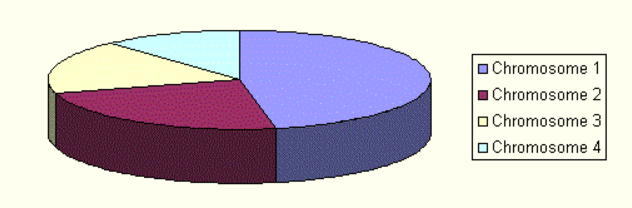
\includegraphics[width=\textwidth]{partials/graphics/roulette.png}
  \caption{Model over roulette metoden.\footfullcite{roulette}}
  \label{fig:roulette}
\end{figure}

\subsubsection{Rang metoden}
I rang metoden bliver individerne sorteret efter størrelsen på deres fitness. Derefter bliver individerne tildelt lodder efter den plads de har fået efter sorteringen. Det vil sige at det individ med den laveste fitness får tildelt et lod, den med den anden mindste får tildelt to lodder osv.. Antallet af lodder et individ er blevet tildelt forstørre chancen for at individet bliver valgt som forældre til en fremtidig generation. I modsætning til roulette metoden, har fitnessen altså i rang metoden en indirekte påvirkning på individernes chance for at bliver valgt.\footfullcite{jebari2013}

\subsubsection{Tournament metoden}
To tilfældige individer bliver valgt fra populationen. En tilfældig værdi fra 0-1 genereres for at sammenligne den med valgte sandsynlighedsværdi. Hvis værdien er mindre eller lige med sandsynlighedsværdien, bliver det individ med højst fitness valgt ellers bliver individet med den lavere fitness valgt. Sandsynlighedsværdien bliver altid sat højere end 0.5 for at favorisere individet med den højeste fitness.\footfullcite{jebari2013}
\\\\
I det følgende program benyttes roulette metoden. Ved brug af roulette metoden er der forskel ved sammenligning af to individer, hvor deres fitness ligger tæt på hinanden, og to individer hvor deres fitness ligger langt fra hinanden. Tournemant metoden laver ikke nogle forskel på disse situationer og er derfor ikke optimal til dette problem.

\subsection{Produktafgrænsning}
  Et godt skema stiller store krav til et skemalægningsprogram. Det er vigtigt at programmet er i stand til at møde disse krav, ellers er programmet essentielt ubrugeligt. Det grundlæggende princip i programmet er, at automatiserer skemalægningsprocessen ud fra forudbestemte parametre. Grundet den begrænsede tid, der er afsat til dette projekt, vil følgende afsnit afgrænse hvilke funktionaliteter, som vil blive løst i det endelige program.

Som tidligere nævnt vil programmets selektion være baseret på genetiske algoritmer. Brugen af genetiske algoritmer giver mulighed for at buge programmet gentagende gange med forskellige resultater. En bruger kan køre programmet indtil, der genereres et skema, de anser som tilfredsstillende.

Programmet skal tage højde for hvilke prædefineret krav, både lovmæssige og brugerspecifikke.

De lovmæssige krav er defineret i afsnittet om lovgivning. Der er ikke meget debat om at disse krav er essentielle grundsten, og derfor skal inkluderes for at lave et acceptabelt program. 

I interviewet med Søren Kusk blev konkrete problemer understeget. Forberedelses timer til lærerne, som ligger samlet, tunge fag skal ligge før middag, tværfaglig undervisning på tværs af klasser.\footfullcite{interview}

Programmet skal arbejde med at løse de tre problemer. Som nævnt i problemafgrænsningen er samlede forberedelsestimer et vigtigt krav at få opfyldt. Det er vigtigt for lærerne at have tilstrækkelig konsekutive forberedelses timer, så undervisningstimerne er af tilstrækkelig kvalitet for elevernes indlæring. Det er derfor medtaget i programmet, som et at de primære problemer, som skal løses. 

Et andet problem der er valgt til at løse, er problemet omkring tunge fag efter middag. Dette var et problem, som var blevet gjort til kende af Søren Kusk og som en præference, der ønskes at medtages i skemalægningen.\footfullcite{interview} Det er derfor også et krav, som vælges at tages højde for i forhold til programmet, både på grund af det var et problem værd at nævne af Søren Kusk, men ydermere et koncept genetiske algoritmer har potentiale til at løse ved hjælp af selektion og nedprioritering af skemaer med sådanne hændelser.

Sidste prioritet fra interviewet som vælges at programmet skal tage højde for, er kravet om tværfaglige undervisning på tværs af parallelklasserne. Der stilles krav om, at lærerne kan undervise parallelklasser samtidig. Dette er dog kun muligt, hvis to eller mere parallelklasser har det samme fag samtidig. Derfor skal programmet være i stand til vurdere placeringen af specifikke fag og lærere på tværs af parallelklasser. 

Disse krav er lavet ud fra interviewet, men yderligere krav blev opstillet. Kravene er som følgende:

Sofiendalskolen ønsker ikke at have mere end to blokke med samme fag i træk. \footfullcite{interview}

Programmet skal være i stand til at lave et mængde skemaer for flere klasser. Grundet omfanget af dette krav og den tidsmæssige begrænsning, der ligger på dette projekt, er valget truffet om at begrænse dette krav til 7. 8. og 9. klasse. 

Fritimer skal ligge i slutningen af dagen og bestemt ikke i midten af dagen. Dette er gjort for ikke, at forlænge skoledagen længere end nødvendigt, ydermere ikke have længere pauser, som kan lede i brud af koncentrationen hos eleverne.

Programmet skal bruge en fil, som simulerer brugerinput. Valget er taget som et alternativ til en brugergrænseflade.  


\subsection{Kravspecifikationer}
  Hvilke krav og bindinger skal vægtes i programmet:


•	Programmet skal generere skemaer for 9 klasser, 3 skemaer for henholdsvis 7, 8 og 9 klassetrin.


•	Programmet skal overholde minimumskravene for timetal i folkeskolen.


•	Programmet skal tage højde for at klassetrinene ikke har det samme antal fag eller samme type fag.


•	Det skal ikke være muligt for en lærer at have lektioner i to klasser på en gang.


•	Lærerne skal have mere end en forberedelsestime adgangen.


•	Der må ikke være tomme lektioner i midten eller starten af skemaet.


•	Samarbejde på tværs af parallelklasserne skal være muligt. 


•	Programmet skal læse lærernes initialer ind via en fil. Filen skal simulere en indstillingsmenu for forbrugeren.


•	Der må højest være 8 lektioner på en dag.


•	Lektionerne skal helst være ligeligt fordelt over alle ugedagene, således at der ikke er 3 dage med 8 lektioner og 2 dage med 4 lektioner.


\subsection{Kodestil}
  I programmet anvendes en række defines i toppen, hvor værdierne kan ændres efter behov. Så er de forskellige skolefag skrevet som en enumeration type, efterfulgt af definitioner på de anvendte structs. Herefter ligger alle anvendte funktioner som prototyper. Selve funktionerne ligger i bunden. Kommentarer skrives over det stykke kode den forklarer. Når der udføres en algoritme i en funktion eller en løkke, er algoritmen rykket ind med et tab af to mellemrum. Tuborgklammer starter inden linjeskift, efter funktioner og løkker, og afsluttes efter et linjeskift. 